\begin{frame}
    \frametitle{\problemtitle}

    \begin{itemize}
        \item Determine whether it is possible to hit all rooms in a spaceship with a single, infinite-length beam.
        \item The spaceship is represented by a set of $1 \leq n \leq 2 \cdot 10^5$
        axis-aligned non-intersecting rectangles (${0\leq x_1<x_2\leq10^9}$ and ${0\leq y_1<y_2\leq10^9}$).
    \end{itemize}

    \vfill

    \centering
    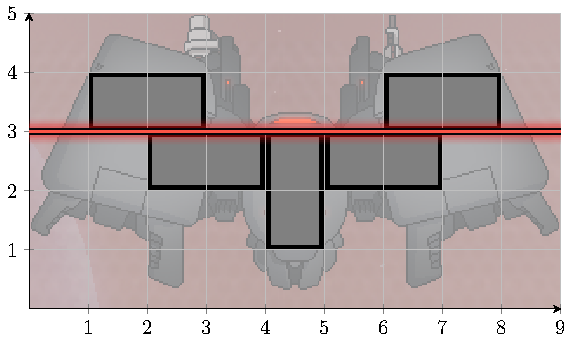
\includegraphics[height=0.4\textheight]{sample}

    \small
    Illustration of Sample Input 1, which consists of five grey rooms.
    The hull beam in red hits all rooms and is the only valid solution in this case.
\end{frame}
